% Copyright (C) 2020 - Michael Baudin

\documentclass{beamer}

%\setbeameroption{hide notes}
%\setbeameroption{show notes}
%\setbeameroption{show only notes}

% Copyright (C) 2012 - EDF R&D - Michael Baudin

% To highlight source code
\usepackage{listings}
\definecolor{darkgreen}{rgb}{0,0.5,0}
\definecolor{violet}{rgb}{0.5,0,1}

\usepackage{algorithm,algorithmic}
\usepackage{bbm}

\usepackage{lmodern}% http://ctan.org/pkg/lm

\usetheme{Montpellier}
\setbeamertemplate{navigation symbols}{} % Remove navigation
\useoutertheme{infolines}

\usepackage[utf8]{inputenc}
\usepackage[T1]{fontenc}

%\usepackage[french]{babel}
%\uselanguage{French}
%\languagepath{French}

\def\bx{{\bf x}}
\def\RR{\mathbb{R}}

\newcommand{\pyvar}[1]{\texttt{#1}}

\def \ot {OpenTURNS}

\hypersetup{colorlinks=true}

\lstset{
  % general command to set parameter(s)
   %basicstyle=\footnotesize\ttfamily, %
   %basicstyle=\normalsize \ttfamily, %
   basicstyle=\scriptsize\ttfamily, %
   keywordstyle=\color{violet}\bfseries,%
   commentstyle=\color{darkgreen}\bfseries,%
   showspaces=false,%
   stringstyle=\color{red}\bfseries, 
   otherkeywords={NumericalMathFunction, Gumbel, Normal, TruncatedDistribution, %
       CompositeRandomVector, Uniform, PythonFunction, ComposedDistribution, RandomVector, %
	   Event, MonteCarlo, NumericalSample, IntervalMesher, Field, HistogramFactory, %
	   Graph, BoxCoxFactory, CompositeProcess, Indices, WhittleFactory, ARMAFactory, %
	   Basis, TrendFactory, BoxCoxTransform, SpatialFunction, TimeSeries, %
	   WelchFactory, GreaterOrEqual, SymbolicFunction, IndependentCopula, %
	   FORM, Cobyla, getResult, getEventProbability, run, drawImportanceFactors},
}

\newcommand{\fcar}[2] {{\mathbbm{1}}_{#1}\left(#2\right)}
\newcommand{\vect}[1]{{\underline{#1}}}
\newcommand{\idx}{\vect{\alpha}}
\newcommand{\argmin}{\operatornamewithlimits{argmin}}


\title[PERSALYS]{PERSALYS, the graphical interface of OpenTURNS}

<<<<<<< HEAD
\author[Baudin et al.]{
=======
\author[PERSALYS Team]{
<<<<<<< HEAD
<<<<<<< HEAD
>>>>>>> b408b51... Draft of UD Persalys slides.
Micha�l Baudin \inst{1} \and
=======
Michaël Baudin \inst{1} \and
>>>>>>> d198f90... Add slides from 2019. Add figures.
Thibault Delage \inst{1} \and
Antoine Dumas \inst{2} \and \\
Anne Dutfoy \inst{1} \and
Guillaume Garcia \inst{2} \and
Anthony Geay \inst{1} \and \\
Ovidiu Mircescu \inst{1} \and
Aurélie Ladier \inst{2} \and
Julien Schueller \inst{2} \and  \\
Thierry Yalamas \inst{2}
=======
M. Baudin \inst{1} \and
T. Delage \inst{1} \and
A. Dumas \inst{2} \and
A. Dutfoy \inst{1} \and \\
G. Garcia \inst{2} \and
A. Geay \inst{1} \and
O. Mircescu \inst{1} \and
A. Ladier \inst{2} \and \\
J. Schueller \inst{2} \and
T. Yalamas \inst{2}
>>>>>>> 01c5443... Shorten author names
}

\institute[EDF-Phiméca]{
\inst{1} EDF R\&D. 6, quai Watier, 78401, Chatou Cedex - France, michael.baudin@edf.fr \and %
\inst{2} Phimeca Engineering. 18/20 boulevard de Reuilly, 75012 Paris - France, yalamas@phimeca.com
}

\date[]{19 June 2020, OpenTURNS User's day}

%%%%%%%%%%%%%%%%%%%%%%%%%%%%%%%%%%%%%%%%%%%%%%%%%%%%%%%%%%%%%%%%%%%%%%%%%%%%%

  \begin{document}

%%%%%%%%%%%%%%%%%%%%%%%%%%%%%%%%%%%%%%%%%%%%%%%%%%%%%%%%%%%%%%%%%%%%%%%%%%%%%

  \begin{frame}
  \titlepage
  
  \begin{columns}
    \column{0.45\textwidth}
  \begin{center}
\includegraphics[height=0.15\textheight]{figures/edf.jpg}
\end{center}
    \column{0.1\textwidth}
	
    \column{0.45\textwidth}
  \begin{center}
\includegraphics[height=0.15\textheight]{figures/logo_phimeca.png}
\end{center}
  \end{columns}

  \end{frame}

\note{
I would like to thank the organizers to inviting us to present our tools. 
}

%%%%%%%%%%%%%%%%%%%%%%%%%%%%%%%%%%%%%%%%%%%%%%%%%%%%%%%%%%%%%%%%%%%%%%%%%%%%%

\begin{frame}
\frametitle{Contents}
\tableofcontents
\end{frame}

%%%%%%%%%%%%%%%%%%%%%%%%%%%%%%%%%%%%%%%%%%%%%%%%%%%%%%%%%%%%%%%%%%%%%%%%%%%%%

\section{Overview}

\begin{frame}
\frametitle{Bring Uncertainty Methodology to Engineers}
\begin{itemize}
\item 4 years ago

\begin{itemize}
\item EDF R\&D wants to maximize the use of OpenTURNS\textregistered{} by its engineer/researcher (and improve an existing GUI) => develop a GUI to make more easy to use

\item Phimeca has already developed an "OpenTURNS GUI" (PhimecaSoft\textregistered{}) which satisfy some needs of EDF R\&D but not all.

\item EDF R\&D and Phimeca decided to start a specific partnership in order to develop a new GUI based on OpenTURNS\textregistered{} and "Salome Tools": Paraview, Yacs, ...
\end{itemize}

\item Persalys is available, on Salome website, in EDF Specific Salome version and commercialized by Phimeca
\end{itemize}
\end{frame}

%%%%%%%%%%%%%%%%%%%%%%%%%%%%%%%%%%%%%%%%%%%%%%%%%%%%%%%%%%%%%%%%%%%%%%%%%%%%%
\begin{frame}
\frametitle{Some expectations regarding the GUI}
\begin{itemize}
\item As easy to use as possible and, when it is possible, a GUI which can guide the user 

\item Possibility to use it inside Salome Platform to 
\begin{itemize}
\item Use supercomputing resources (e.g. Gaïa, 3 052 Tflops peak, 41 000 cores)
\item Connect to EDF numerical code users (Code\_Aster for example)
\end{itemize}

\item Take benefit from the advanced visualization capability from Paraview

\item Drive the GUI from a python script usable in an "expert" mode
\end{itemize}
\end{frame}

%%%%%%%%%%%%%%%%%%%%%%%%%%%%%%%%%%%%%%%%%%%%%%%%%%%%%%%%%%%%%%%%%%%%%%%%%%%%%

\begin{frame}
\frametitle{PERSALYS, the graphical user interface of \ot{}}
	
\begin{itemize}
\item Main goal : provide a graphical interface of 
\ot{} in the SALOME integration platform
\item Features
	\begin{itemize}
	\item Uncertainty quantification : definition of the 
	probabilistic model (including dependence), distribution fitting (including 
	copulas), physical model with vector input 
	and vector output or 1D Fields,
	central tendency, sensitivity analysis, probability estimate, 
	metamodeling (polynomial chaos, kriging), screening (Morris), 
	optimization, design of experiments
	\item Generic (not dedicated to a specific application)
	\item GUI language : English, French
	\end{itemize}

\item Partners : EDF, Phiméca
\item Licence : LGPL

\item Schedule : 
	\begin{itemize}
	\item Since summer 2016, one EDF release per year
	\item On the internet (free) : SALOME\_EDF in the "CONTRIBUTIONS" section 
	since 2018 on \url{https://www.salome-platform.org}
	
	\end{itemize}

\end{itemize}

\end{frame}

\note{
We created a new tool within SALOME, called PERSALYS. 
}



%%%%%%%%%%%%%%%%%%%%%%%%%%%%%%%%%%%%%%%%%%%%%%%%%%%%%%%%%%%%%%%%%%%%%%%%%%%%%

\section{PERSALYS v8: Calibration}


%%%%%%%%%%%%%%%%%%%%%%%%%%%%%%%%%%%%%%%%%%%%%%%%%%%%%%%%%%%%%%%%%%%%%%%%%%%%%

\begin{frame}
\frametitle{Calibration}

Given a physical model $H$, observed inputs $x$, 
observed outputs $y$ we can calibrate $\theta$ so that 
$$
y_i = H(x_i, \theta) + \epsilon
$$
where $\epsilon$ is a random variable.

Calibration outputs:
\begin{itemize}
\item the optimal value $\theta^\star$,
<<<<<<< HEAD
\item the distribution of $\theta^\star$.
=======
\item the distribution of $\theta^\star$,
<<<<<<< HEAD
\item the distribution of the residuals $y_i - H(x_i, \theta)$.
>>>>>>> b408b51... Draft of UD Persalys slides.
=======
\item the distribution of the residuals $r_i = y_i - H(x_i, \theta^\star)$.
>>>>>>> d198f90... Add slides from 2019. Add figures.
\end{itemize}

This allows to get confidence intervals of $\theta^\star$.

\end{frame}

%%%%%%%%%%%%%%%%%%%%%%%%%%%%%%%%%%%%%%%%%%%%%%%%%%%%%%%%%%%%%%%%%%%%%%%%%%%%%

\begin{frame}
\frametitle{Calibration}

In PERSALYS, this requires:
\begin{itemize}
\item a physical model $H$, 
\item a data file containing the observed inputs and outputs.
\end{itemize}

\begin{center}
\includegraphics[width=0.4\textwidth]{figures/observations_contextMenu.png}
\end{center}

\end{frame}

%%%%%%%%%%%%%%%%%%%%%%%%%%%%%%%%%%%%%%%%%%%%%%%%%%%%%%%%%%%%%%%%%%%%%%%%%%%%%

\begin{frame}
\frametitle{Calibration}
	
\begin{center}
\includegraphics[width=0.7\textwidth]{figures/S94-Calibration_parameters.png}
\end{center}

\end{frame}


%%%%%%%%%%%%%%%%%%%%%%%%%%%%%%%%%%%%%%%%%%%%%%%%%%%%%%%%%%%%%%%%%%%%%%%%%%%%%

\begin{frame}
\frametitle{Calibration}
	
\begin{center}
\includegraphics[width=0.9\textwidth]{figures/S94-Parametres.png}
\end{center}

\end{frame}

%%%%%%%%%%%%%%%%%%%%%%%%%%%%%%%%%%%%%%%%%%%%%%%%%%%%%%%%%%%%%%%%%%%%%%%%%%%%%

\begin{frame}
\frametitle{Calibration}
	
\begin{center}
\includegraphics[width=0.9\textwidth]{figures/S94-Calage-Gaussien-prior.png}
\end{center}

\end{frame}

%%%%%%%%%%%%%%%%%%%%%%%%%%%%%%%%%%%%%%%%%%%%%%%%%%%%%%%%%%%%%%%%%%%%%%%%%%%%%

\begin{frame}
\frametitle{Calibration}
	
\begin{center}
<<<<<<< HEAD
\includegraphics[width=0.7\textwidth]{figures/calibration_ResultWindow.png}
=======
\includegraphics[width=0.7\textwidth]{figures/calibration-ks-zv-zm-optimal.png}
>>>>>>> b408b51... Draft of UD Persalys slides.
\end{center}

\end{frame}

%%%%%%%%%%%%%%%%%%%%%%%%%%%%%%%%%%%%%%%%%%%%%%%%%%%%%%%%%%%%%%%%%%%%%%%%%%%%%

\begin{frame}
\frametitle{Calibration}
	
<<<<<<< HEAD
TODO : PDF de $\theta$ -> capture d'�cran par Thibault ?
=======
\begin{center}
\includegraphics[width=0.7\textwidth]{figures/calibration-Zv-prior-posterior.png}
\end{center}
>>>>>>> b408b51... Draft of UD Persalys slides.

\end{frame}

%%%%%%%%%%%%%%%%%%%%%%%%%%%%%%%%%%%%%%%%%%%%%%%%%%%%%%%%%%%%%%%%%%%%%%%%%%%%%

\begin{frame}
\frametitle{Calibration}
	
\begin{center}
<<<<<<< HEAD
\includegraphics[width=0.9\textwidth]{figures/S94-Resultat-3DVAR.png}
=======
\includegraphics[width=0.7\textwidth]{figures/calibration-residual-analysis.png}
>>>>>>> b408b51... Draft of UD Persalys slides.
\end{center}

\end{frame}

\note{
Rouge : la distribution des résidus avant calage.
Vert : la distribution des résidus après calage.
Bleu : la distribution gaussienne des résidus. Gaussien (TODO : préciser)
}

%%%%%%%%%%%%%%%%%%%%%%%%%%%%%%%%%%%%%%%%%%%%%%%%%%%%%%%%%%%%%%%%%%%%%%%%%%%%%

<<<<<<< HEAD
\section{TODO}

\begin{frame}
\frametitle{TODO}
	
\begin{itemize}
\item Couping tools
\item website ?
=======
\section{Coupling tools}

\begin{frame}
\frametitle{Coupling with external code}

A new physical coupling dialog was created:
\begin{itemize}
\item Execute any computer code from system
\item Create a pipeline of commands
\item Exchange data with files
\item Manage input and output cache to save simulations
\item Can be parallel : multithread or distributed (in SALOME)
>>>>>>> b408b51... Draft of UD Persalys slides.
\end{itemize}

\end{frame}

%%%%%%%%%%%%%%%%%%%%%%%%%%%%%%%%%%%%%%%%%%%%%%%%%%%%%%%%%%%%%%%%%%%%%%%%%%%%%
<<<<<<< HEAD
=======

\begin{frame}
\frametitle{Coupling with external code}

\begin{center}
\includegraphics[width=0.7\textwidth]{figures/coupling-input-focus.png}
\end{center}

\end{frame}

%%%%%%%%%%%%%%%%%%%%%%%%%%%%%%%%%%%%%%%%%%%%%%%%%%%%%%%%%%%%%%%%%%%%%%%%%%%%%

\begin{frame}
\frametitle{Coupling with external code}

Resources are files to copy to run the simulation : mesh, parameters, etc...

\begin{center}
\includegraphics[width=0.7\textwidth]{figures/coupling-ressources-focus.png}
\end{center}

\end{frame}

%%%%%%%%%%%%%%%%%%%%%%%%%%%%%%%%%%%%%%%%%%%%%%%%%%%%%%%%%%%%%%%%%%%%%%%%%%%%%

\begin{frame}
\frametitle{Coupling with external code}

\begin{center}
\includegraphics[width=0.8\textwidth]{figures/coupling-output-focus.png}

\includegraphics[width=0.8\textwidth]{figures/coupling-cache-focus.png}
\end{center}

\end{frame}

%%%%%%%%%%%%%%%%%%%%%%%%%%%%%%%%%%%%%%%%%%%%%%%%%%%%%%%%%%%%%%%%%%%%%%%%%%%%%

\section{Website}

\begin{frame}
\frametitle{Website}

\url{persalys.fr} : download (source, binaries), doc (videos tutorials), news
	
\begin{center}
\includegraphics[width=0.6\textwidth]{figures/persalys-web.png}
\end{center}

\end{frame}

%%%%%%%%%%%%%%%%%%%%%%%%%%%%%%%%%%%%%%%%%%%%%%%%%%%%%%%%%%%%%%%%%%%%%%%%%%%%%
>>>>>>> b408b51... Draft of UD Persalys slides.
\section{What's next ?}

\begin{frame}
\frametitle{What's next ?}
  \begin{columns}
    \column{0.5\textwidth}

PERSALYS Roadmap : 
\begin{itemize}
<<<<<<< HEAD
\item Calibration
=======
>>>>>>> b408b51... Draft of UD Persalys slides.
\item 2D Fields, 3D Fields
\item In-Situ fields based on the MELISSA library (with INRIA): 
when we cannot store the whole sample in memory or on the hard drive, 
update the statistics (e.g. the mean, Sobol' indices) sequentially, 
with distributed computing. 
\end{itemize}

    \column{0.5\textwidth}

\begin{center}
\includegraphics[height=0.5\textheight]{figures/image034.png}
\end{center}

	\end{columns}

\end{frame}

\note{
We are currently working on adding features to perform 
the calibration of a computer code (almost done). 

The next features we plan to add to PERSALYS are the management 
of 2D and 3D stochastic fields. 

We also work on the use of the MELISSA software which performs 
in-situ studies. 

This library allows to perform UQ studies in situations 
where we cannot store more than a couple of multidimensional fields 
in memory or on the hard drive. 
}

%%%%%%%%%%%%%%%%%%%%%%%%%%%%%%%%%%%%%%%%%%%%%%%%%%%%%%%%%%%%%%%%%%%%%%%%%%%%%

\begin{frame}
\frametitle{The end}

\begin{center}
Thanks !
\end{center}

\begin{center}
Questions ?
\end{center}

\end{frame}

\note{
Thank you for your attention. 

If you have any question, it would be a pleasure to answer them. 

If you want a live demo of PERSALYS, I can show you during the coffee break.
}

%%%%%%%%%%%%%%%%%%%%%%%%%%%%%%%%%%%%%%%%%%%%%%%%%%%%%%%%%%%%%%%%%%%%%%%%%%%%%

\begin{frame}
\frametitle{PERSALYS: estimate the parameters of the copulas}
	

  \begin{columns}
    \column{0.4\textwidth}
	
\begin{itemize}
\item Inference of the dependence of the multivariate sample 
\item Guided choice according to the BIC and Kendall plot
\end{itemize}

    \column{0.6\textwidth}

\begin{center}
\includegraphics[width=0.95\textwidth]{figures/persalys-copula-inference.png}
\end{center}

	\end{columns}


\end{frame}

\note{
To estimate the parameters of a copula, you can perform the inference of a 
multivariate sample. 
}

% %%%%%%%%%%%%%%%%%%%%%%%%%%%%%%%%%%%%%%%%%%%%%%%%%%%%%%%%%%%%%%%%%%%%%%%%%%%%%

%\section{PERSALYS, the graphical user interface}

\begin{frame}
\frametitle{SALOME}

  \begin{columns}
    \column{0.5\textwidth}
	
\begin{itemize}
\item Integration platform for pre and post processing, and 2D/3D numerical simulation 
\item Features : geometry, mesh, distributed computing
\item Visualization, data assimilation, uncertainty treatment
\item Partners : EDF, CEA, Open Cascade
\item Licence : LGPL
\item Linux, Windows
\item \url{www.salome-platform.org}
\end{itemize}

    \column{0.5\textwidth}

\begin{center}
\includegraphics[width=0.95\textwidth]{figures/Salome-hydro-platform}
\end{center}

	\end{columns}
\end{frame}

\note{
Before presenting the graphical user interface, I would like to say some 
words about SALOME.
}

%%%%%%%%%%%%%%%%%%%%%%%%%%%%%%%%%%%%%%%%%%%%%%%%%%%%%%%%%%%%%%%%%%%%%%%%%%%%%

\begin{frame}[containsverbatim]
\frametitle{OpenTURNS: estimate Sobol' indices sequentially}

Part 2 : Estimate Sobol' sensitivity indices with an incremental algorithm.
\begin{itemize}
\item Let us denote by $\Phi_k^F$ (resp. $\Phi_k^T$) the cumulated 
distribution function of the gaussian distribution of the first (resp. total) 
order sensitivity indice of the k-th input variable.

\item We set $\alpha\in[0,1]$ a quantile level and $\epsilon \in(0,1]$ a quantile precision. 

\item The algorithms stops when, on all components, first and total order 
indices haved been estimated with enough precision.
 
The precision is said to be sufficient if 
$$
\Phi_k^F(1-\alpha) - \Phi_k^F(\alpha) \leq \epsilon
$$
and 
$$
\Phi_k^T(1-\alpha) - \Phi_k^T(\alpha) \leq \epsilon
$$
for $k=1,...,n_X$. 

\end{itemize}

\end{frame}

\note{
We now define the stopping criteria. 
}
%%%%%%%%%%%%%%%%%%%%%%%%%%%%%%%%%%%%%%%%%%%%%%%%%%%%%%%%%%%%%%%%%%%%%%%%%%%%%

\begin{frame}
\frametitle{PERSALYS: 1D fields}
	
\begin{itemize}
\item Karhunen Loeve decomposition
\item Show modes, eigenvalues and projection coefficients
\end{itemize}

\begin{center}
\includegraphics[width=0.45\textwidth]{figures/persalys-field-modes.png}
\includegraphics[width=0.45\textwidth]{figures/persalys-field-plotmatrix-extract.png}
\end{center}

\end{frame}
%%%%%%%%%%%%%%%%%%%%%%%%%%%%%%%%%%%%%%%%%%%%%%%%%%%%%%%%%%%%%%%%%%%%%%%%%%%%%
%\section{Extra slides}

\begin{frame}
\frametitle{Interactive uncertainty visualization with Paraview}

\begin{center}
\includegraphics[width=0.9\textwidth]{figures/image032.png}
\end{center}

\end{frame}

%%%%%%%%%%%%%%%%%%%%%%%%%%%%%%%%%%%%%%%%%%%%%%%%%%%%%%%%%%%%%%%%%%%%%%%%%%%%%

\begin{frame}
\frametitle{Methodology}

\begin{center}
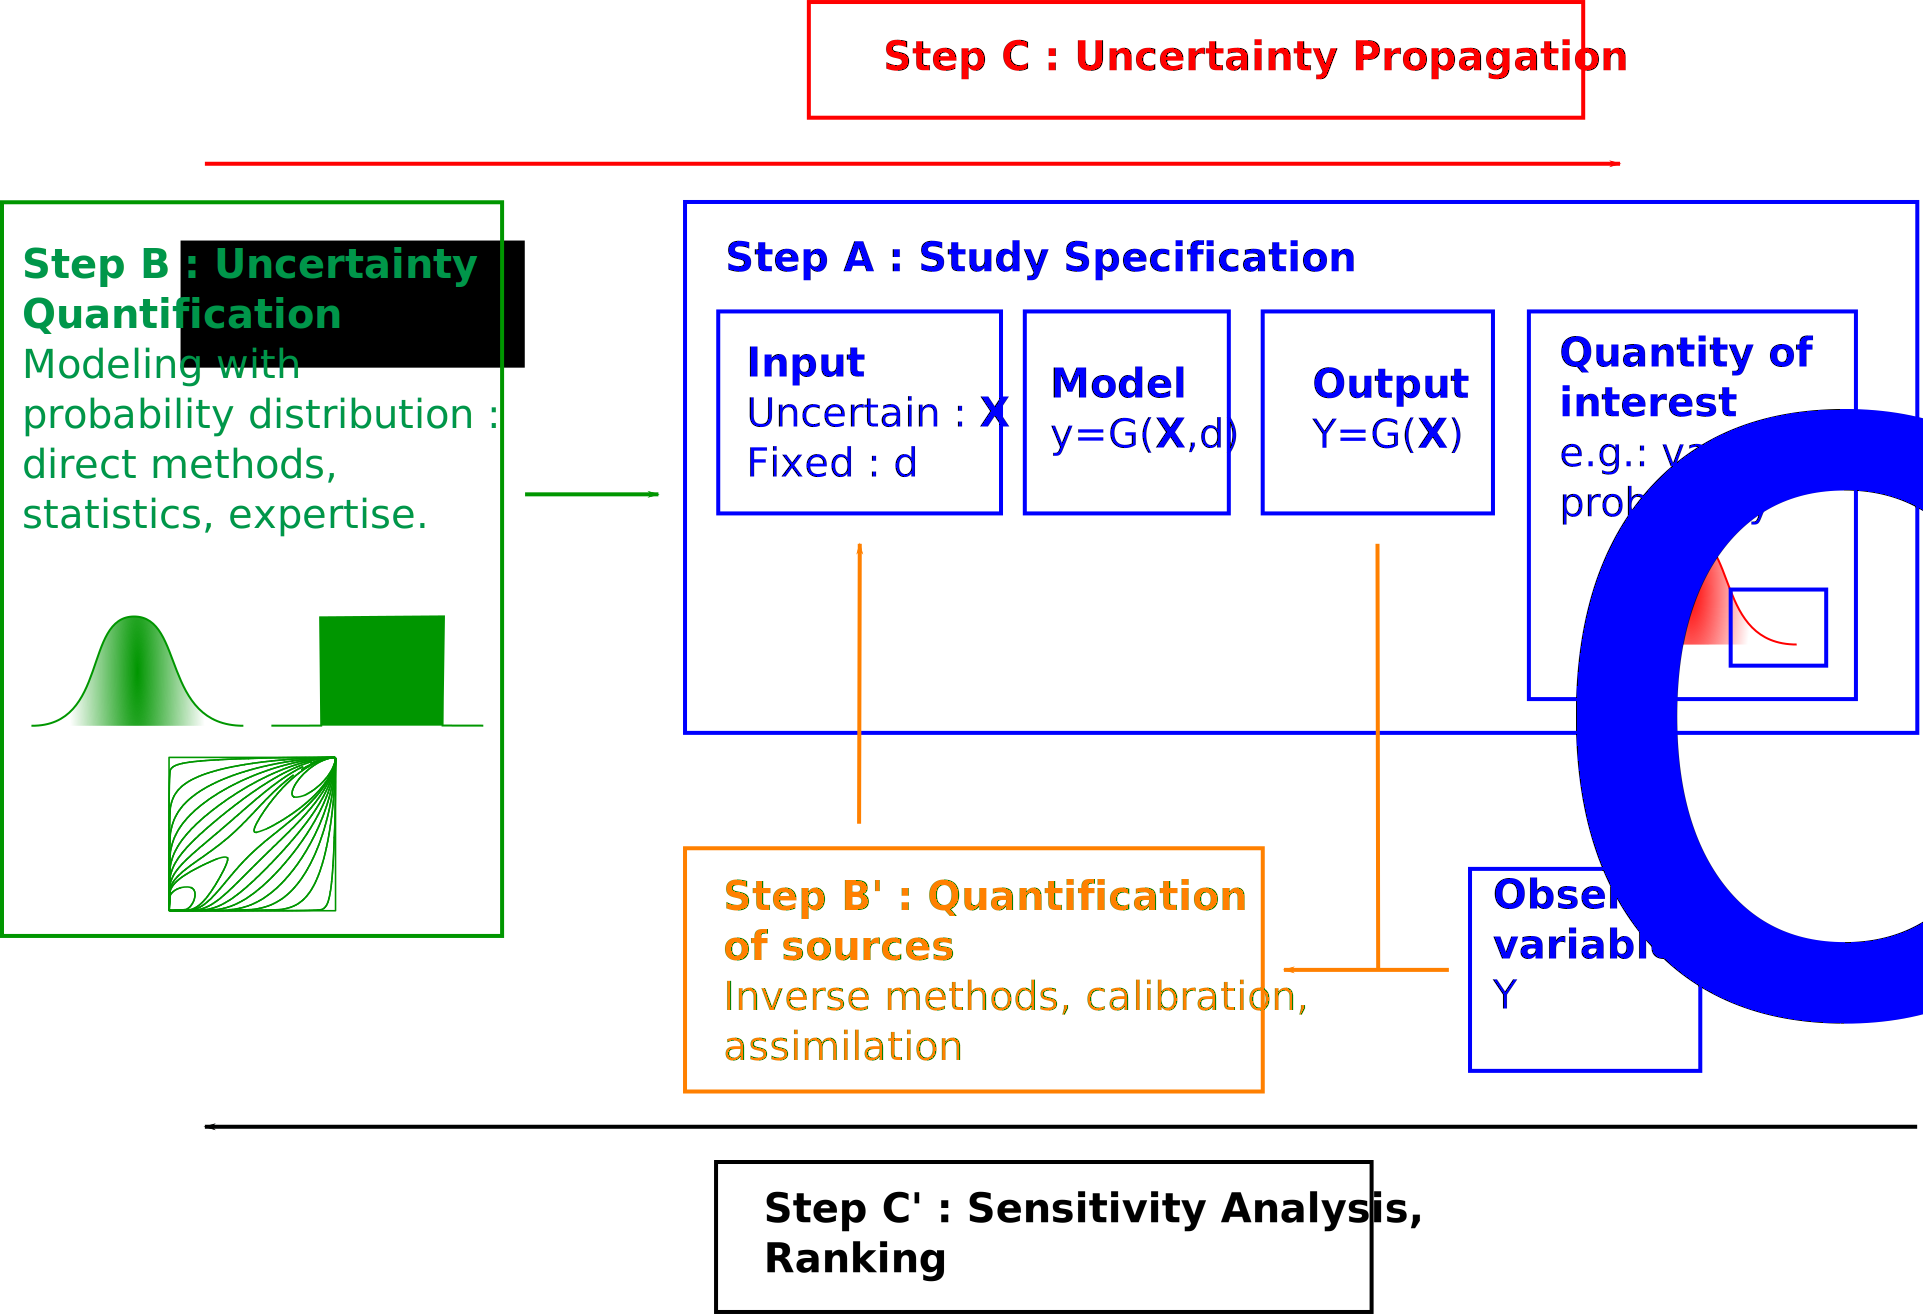
\includegraphics[width=0.9\textwidth]{figures/MethodologieIncertitude-EN.pdf}
\end{center}

\end{frame}

%%%%%%%%%%%%%%%%%%%%%%%%%%%%%%%%%%%%%%%%%%%%%%%%%%%%%%%%%%%%%%%%%%%%%%%%%%%%%

\begin{frame}
\frametitle{Software architecture}

  \begin{columns}
    \column{0.4\textwidth}
	
Two entry points:
\begin{itemize}
\item interactive,
\item Python.
\end{itemize}

Advantages of the Python programming of the GUI:
\begin{itemize}
\item unit tests,
\item going beyond the GUI
\end{itemize}

    \column{0.6\textwidth}

\begin{center}

\includegraphics[width=0.95\textwidth]{figures/ArchiGUI-Internal.pdf}
\end{center}

	\end{columns}

\begin{center}
\includegraphics[width=0.9\textwidth]{figures/image007.png}
\end{center}

\end{frame}

%%%%%%%%%%%%%%%%%%%%%%%%%%%%%%%%%%%%%%%%%%%%%%%%%%%%%%%%%%%%%%%%%%%%%%%%%%%%%
%\section{Demo backup}

%%%%%%%%%%%%%%%%%%%%%%%%%%%%%%%%%%%%%%%%%%%%%%%%%%%%%%%%%%%%%%%%%%%%%%%%%%%%%

\begin{frame}
\frametitle{Symbolic physical model}

\begin{center}
\includegraphics[width=0.9\textwidth]{figures/image009.png}
\end{center}

\end{frame}

%%%%%%%%%%%%%%%%%%%%%%%%%%%%%%%%%%%%%%%%%%%%%%%%%%%%%%%%%%%%%%%%%%%%%%%%%%%%%

\begin{frame}
\frametitle{Probabilistic model}

\begin{center}
\includegraphics[height=0.8\textheight]{figures/image013.png}
\end{center}

\end{frame}

%%%%%%%%%%%%%%%%%%%%%%%%%%%%%%%%%%%%%%%%%%%%%%%%%%%%%%%%%%%%%%%%%%%%%%%%%%%%%

\begin{frame}
\frametitle{Limit state study : definition of the threshold}

\begin{center}
\includegraphics[width=0.4\textwidth]{figures/image015.png}
\end{center}

\end{frame}

%%%%%%%%%%%%%%%%%%%%%%%%%%%%%%%%%%%%%%%%%%%%%%%%%%%%%%%%%%%%%%%%%%%%%%%%%%%%%

\begin{frame}
\frametitle{Limit state study : algorithm parameters}

\begin{center}
\includegraphics[width=0.95\textwidth]{figures/image017.png}
\end{center}

\end{frame}

%%%%%%%%%%%%%%%%%%%%%%%%%%%%%%%%%%%%%%%%%%%%%%%%%%%%%%%%%%%%%%%%%%%%%%%%%%%%%

\begin{frame}
\frametitle{Limit state study : summary}

\begin{center}
\includegraphics[width=0.7\textwidth]{figures/image019.png}
\end{center}

\end{frame}

%%%%%%%%%%%%%%%%%%%%%%%%%%%%%%%%%%%%%%%%%%%%%%%%%%%%%%%%%%%%%%%%%%%%%%%%%%%%%

\begin{frame}
\frametitle{Limit state study : histogram}

\begin{center}
\includegraphics[width=0.7\textwidth]{figures/image021.png}
\end{center}

\end{frame}

%%%%%%%%%%%%%%%%%%%%%%%%%%%%%%%%%%%%%%%%%%%%%%%%%%%%%%%%%%%%%%%%%%%%%%%%%%%%%

\begin{frame}
\frametitle{Central tendency : algorithm parameters}

\begin{center}
\includegraphics[width=0.8\textwidth]{figures/image023.png}
\end{center}

\end{frame}

%%%%%%%%%%%%%%%%%%%%%%%%%%%%%%%%%%%%%%%%%%%%%%%%%%%%%%%%%%%%%%%%%%%%%%%%%%%%%

\begin{frame}
\frametitle{Central tendency : summary results}

\begin{center}
\includegraphics[width=0.8\textwidth]{figures/image025-bottom.png}
\end{center}

\end{frame}

%%%%%%%%%%%%%%%%%%%%%%%%%%%%%%%%%%%%%%%%%%%%%%%%%%%%%%%%%%%%%%%%%%%%%%%%%%%%%

\begin{frame}
\frametitle{Central tendency : summary results}

\begin{center}
\includegraphics[height=0.8\textheight]{figures/image025-top.png}
\end{center}

\end{frame}

%%%%%%%%%%%%%%%%%%%%%%%%%%%%%%%%%%%%%%%%%%%%%%%%%%%%%%%%%%%%%%%%%%%%%%%%%%%%%

\begin{frame}
\frametitle{Central tendency : scatter plots}

\begin{center}
\includegraphics[width=0.8\textwidth]{figures/image028.png}
\end{center}

\end{frame}


%%%%%%%%%%%%%%%%%%%%%%%%%%%%%%%%%%%%%%%%%%%%%%%%%%%%%%%%%%%%%%%%%%%%%%%%%%%%%

\begin{frame}
\frametitle{Sensitivity analysis : Sobol' indices}

\begin{center}
\includegraphics[height=0.8\textheight]{figures/image030.png}
\end{center}

\end{frame}

% %%%%%%%%%%%%%%%%%%%%%%%%%%%%%%%%%%%%%%%%%%%%%%%%%%%%%%%%%%%%%%%%%%%%%%%%%%%%%

\begin{frame}[containsverbatim]
\frametitle{OpenTURNS: estimate the mean}

See the Jupyter Notebook.

\scriptsize{

\lstset{language=python}
\begin{lstlisting}
from openturns.viewer import View
import openturns as ot
from math import sqrt

ot.RandomGenerator.SetSeed(0)

# 1. The function G
def functionCrue(X) :
    Q, Ks, Zv, Zm = X
    alpha = (Zm - Zv)/5.0e3
    H = (Q/(Ks*300.0*sqrt(alpha)))**(3.0/5.0)
    S = [H + Zv - (55.5 + 3.0)]
    return S

# Creation of the problem function
g = ot.PythonFunction(4, 1, functionCrue) 
g = ot.MemoizeFunction(g)
\end{lstlisting}

}

\end{frame}

% %%%%%%%%%%%%%%%%%%%%%%%%%%%%%%%%%%%%%%%%%%%%%%%%%%%%%%%%%%%%%%%%%%%%%%%%%%%%%

\begin{frame}[containsverbatim]
\frametitle{OpenTURNS: estimate the mean}

\begin{columns}
    \column{0.65\textwidth}

\scriptsize{

\lstset{language=python}
\begin{lstlisting}
# 2. Random vector definition
myParamQ = ot.GumbelAB(1013., 558.)
Q = ot.ParametrizedDistribution(myParamQ)
otLOW = ot.TruncatedDistribution.LOWER
Q = ot.TruncatedDistribution(Q, 0, otLOW)
Ks = ot.Normal(30.0, 7.5)
Ks = ot.TruncatedDistribution(Ks, 0, otLOW)
Zv = ot.Uniform(49.0, 51.0)
Zm = ot.Uniform(54.0, 56.0)

# 3. View the PDF
Q.setDescription(["Q (m3/s)"])
View(Q.drawPDF()).show()
\end{lstlisting}

}

\column{0.35\textwidth}
	\begin{center}
	\includegraphics[width=0.95\textwidth]{figures/Q.pdf}
	\end{center}


\end{columns}

\end{frame}

% %%%%%%%%%%%%%%%%%%%%%%%%%%%%%%%%%%%%%%%%%%%%%%%%%%%%%%%%%%%%%%%%%%%%%%%%%%%%%

\begin{frame}[containsverbatim]
\frametitle{OpenTURNS: estimate the mean}


\scriptsize{

\lstset{language=python}
\begin{lstlisting}
# 4. Create the joint distribution function, 
#    the output and the event. 
X = ot.ComposedDistribution([Q, Ks, Zv, Zm])
Y = ot.RandomVector(g, ot.RandomVector(X))

# 5. Estimate expectation with simple Monte-Carlo
sampleSize = 10000
sampleX = X.getSample(sampleSize)
sampleY = g(sampleX)
sampleMean = sampleY.computeMean()
print("Mean=%f" % (sampleMean[0]))
\end{lstlisting}

Output: 
\begin{lstlisting}
Mean by MC =-5.937845
\end{lstlisting}

}

\end{frame}

%%%%%%%%%%%%%%%%%%%%%%%%%%%%%%%%%%%%%%%%%%%%%%%%%%%%%%%%%%%%%%%%%%%%%%%%%%%%%

%\section{Demo}

\begin{frame}
\frametitle{GUI : the demo}

\begin{center}
Demo time.
\end{center}

\end{frame}

%%%%%%%%%%%%%%%%%%%%%%%%%%%%%%%%%%%%%%%%%%%%%%%%%%%%%%%%%%%%%%%%%%%%%%%%%%%%%


\begin{frame}
\frametitle{GUI : outline}

\begin{itemize}
\item From scratch : 3 inputs, 2 outputs, sum, central dispersion study with default parameters
\item Open axialStressedBeam-python.xml : central dispersion with sample size 1000, Threshold P(G<0) with CV=0.05
\item Import crue-4vars-analytique.py : S.A. with sample size 1000, sort by size
\end{itemize}

\end{frame}


%%%%%%%%%%%%%%%%%%%%%%%%%%%%%%%%%%%%%%%%%%%%%%%%%%%%%%%%%%%%%%%%%%%%%%%%%%%%%
%\section{Background}

\begin{frame}
\frametitle{UQ, the easy way}

Main goal : make UQ easy to use
\begin{itemize}
\item classical user-friendly algorithms with a 
state-of-the-art implementation,
\item default parameters of the algorithms whenever possible,
\item an easy access to the HPC resources,
\item an automated connection to the computer code.
\end{itemize}

Produce standard results :
\begin{itemize}
\item numerical results e.g. tables,
\item classical graphics.
\end{itemize}

\end{frame}

%%%%%%%%%%%%%%%%%%%%%%%%%%%%%%%%%%%%%%%%%%%%%%%%%%%%%%%%%%%%%%%%%%%%%%%%%%%%%

\begin{frame}
\frametitle{Overview (1/2)}

Inputs from the user :
\begin{itemize}
\item Physical model : symbolic, Python code or SALOME component
\item Probabilistic model : joint probability distribution function of the input.
\end{itemize}

Then :
\begin{itemize}
\item Central dispersion: estimates the central dispersion of the output Y (e.g. mean).
\item Threshold probability: estimates the probability that the output exceeds a given
threshold S.
\item Sensitivity analysis: estimates the importance of the inputs to the variability of the output.
\end{itemize}

\end{frame}

%%%%%%%%%%%%%%%%%%%%%%%%%%%%%%%%%%%%%%%%%%%%%%%%%%%%%%%%%%%%%%%%%%%%%%%%%%%%%

\begin{frame}
\frametitle{Overview (2/2)}

Probabilistic modeling :
\begin{itemize}
\item Distribution fitting from a sample
\item Dependence modeling (Gaussian copula)
\end{itemize}

Meta-modeling :
\begin{itemize}
\item Polynomial chaos (full or sparse)
\item Kriging
\end{itemize}

\end{frame}

%%%%%%%%%%%%%%%%%%%%%%%%%%%%%%%%%%%%%%%%%%%%%%%%%%%%%%%%%%%%%%%%%%%%%%%%%%%%%

\begin{frame}
\frametitle{Dependence}
	
  \begin{columns}
    \column{0.4\textwidth}
	
\begin{itemize}
\item Dependence is defined using copulas
\item Define arbitrary groups of dependent variables
\item Available copulas (same as in OT): gaussian, Ali-Mikhail-Haq, 
    Clayton, Farlie-Gumbel-Morgenstern, Frank, Gumbel
\item Dependence inference from a sample : Bayesian Information Criteria (BIC) 
or Kendall plot
\end{itemize}

    \column{0.6\textwidth}

\begin{center}
\includegraphics[width=0.95\textwidth]{figures/persalys-dependence-extract.png}
\end{center}

	\end{columns}

\end{frame}

\note{
To define the dependence in PERSALYS, we use the copula tools available in OpenTURNS. 

The Dependence tab shows the list of input variables: you can create a group 
of dependent variables using the checkbutton and add it to the group. 
}

\begin{frame}
\frametitle{1D fields}
	

\begin{itemize}
\item Mesh definition and visualization
\item Import from text or csv file
\end{itemize}

\begin{center}
\includegraphics[width=0.45\textwidth]{figures/persalys-field-define-mesh.png}
\includegraphics[width=0.45\textwidth]{figures/persalys-field-visualize-mesh-extract.png}
\end{center}

\end{frame}

\note{
The most important new feature is the management of 1D stochastic processes. 
}

%%%%%%%%%%%%%%%%%%%%%%%%%%%%%%%%%%%%%%%%%%%%%%%%%%%%%%%%%%%%%%%%%%%%%%%%%%%%%

\begin{frame}
\frametitle{1D fields}
	
\begin{itemize}
\item Functional model definition and probabilistic model
\item Python or symbolic
\end{itemize}

\begin{center}
\includegraphics[width=0.45\textwidth]{figures/persalys-field-define-python-model-extract.png}
\includegraphics[width=0.45\textwidth]{figures/persalys-field-evaluation.png}
\end{center}

\end{frame}

\note{
The Python function has 4 (four) inputs named z0, v0, m and c. 

Moreover, the Python function depends on the index parameter which name is "t". 

On the right figure, this is what appears when we click on the "Evaluate" button: 
one evaluation of the function is then a trajectory which depends on the time. 
}

%%%%%%%%%%%%%%%%%%%%%%%%%%%%%%%%%%%%%%%%%%%%%%%%%%%%%%%%%%%%%%%%%%%%%%%%%%%%%

\begin{frame}
\frametitle{1D fields}
	
\begin{itemize}
\item Probabilistic model
\item Uncertainty propagation with simple Monte-Carlo sampling
\end{itemize}

\begin{center}
\includegraphics[width=0.45\textwidth]{figures/persalys-field-probabilistic-model.png}
\includegraphics[width=0.45\textwidth]{figures/persalys-field-montecarlo-trajectories-extract.png}
\end{center}

\end{frame}

\note{
Then we can perform the central dispersion analysis of the model. 

On the left, we define the distribution of the input random vector. 

On the right, this is the result of the simulation: a sample made 
of 100 (one hundred) trajectories. 
}
%%%%%%%%%%%%%%%%%%%%%%%%%%%%%%%%%%%%%%%%%%%%%%%%%%%%%%%%%%%%%%%%%%%%%%%%%%%%%

\begin{frame}
\frametitle{1D fields}
	
\begin{itemize}
\item BagChart and Functional Bagchart (from Paraview) 
based on High Density Regions (Hyndman, 1996).
\item To do this, Paraview uses a principal component analysis  
decomposition. 
\item Linked and interactive selections in the views. 
\end{itemize}

\begin{center}
\includegraphics[width=0.45\textwidth]{figures/persalys-field-bagchart.png}
\includegraphics[width=0.45\textwidth]{figures/persalys-field-functional-bagchart.png}
\end{center}

\end{frame}

\note{
To analyze these trajectories requires more advanced tools than with 
classical multivariate samples, so that we can take into account for the 
time dependence. 

We use the BagChart and Functional Bagchart (from Paraview) tools, 
which uses the High Density Regions algorithm . 
}


\end{document}
